%%%%%%%%%%%%%%%%%%%%%%%%%%%%%%%%%%%%%%%%%%%%%%%%%%%%%%%%%%%%%%%%%%%%%%%%%%%%
%\documentclass[a4paper,prc,unsortedaddress,superscriptaddress,showpacs,twocolumn,floatfix]{revtex4}

%\pacs{21.10.-k, 21.10.Tg, 27.20.+n} 
%%%%%%%%%%%%%%%%%%%%%%%%%%%%%%%%%%%%%%%%%%%%%%%%%%%%%%%%%%%%%%%%%%%%%%%%%%%%
%\maketitle
%\section{Experimental setup}
%\label{sec:exp}

%%%%%%%%%%%%%%%%%%%%%%%%%%%%%%%%%%%%%%%%%%%%%%%%%%%%%%%%%%%%%%%%%%%%%%%%%%%%
\section{Motivation}
During the experiment, it was noticed that there was a disagreement between different values of the half-life.
As a side project and as a chance to thoroughly investigate the data, a half-life measurement was taken. 
It has been used in the past for searches of second-class currents.


\section{Half life data analysis}
\label{sec:analysis}

Only the data from the PVT impantation set was used for the half-life analysis.
The rate depedent gain effect causes a larges systematic effect in the CsI(Na) data.

The data was seperated into 6 sets.
The splitting was done by the rates and the gains of the different detectors.
The first and second sets did not have the limiter box installed.
This was to test the effect of the dead time correction across different rates.
Other systematic effect differences were investigated.

In order to do the half-life analysis, software coincidences were imposed.
First, events from the energies and times of each detector were built.
Two conditions were on the energy in the implantation detector and one of the four CsI(Na) detectors.
An additional condition on the time difference between the events recorded in the two detectors. 
A sample spectrum of all the gamma and beta energies is shown in Figure \ref{fig:2DGraph}  

\begin{figure}[!htb]
	\centerline{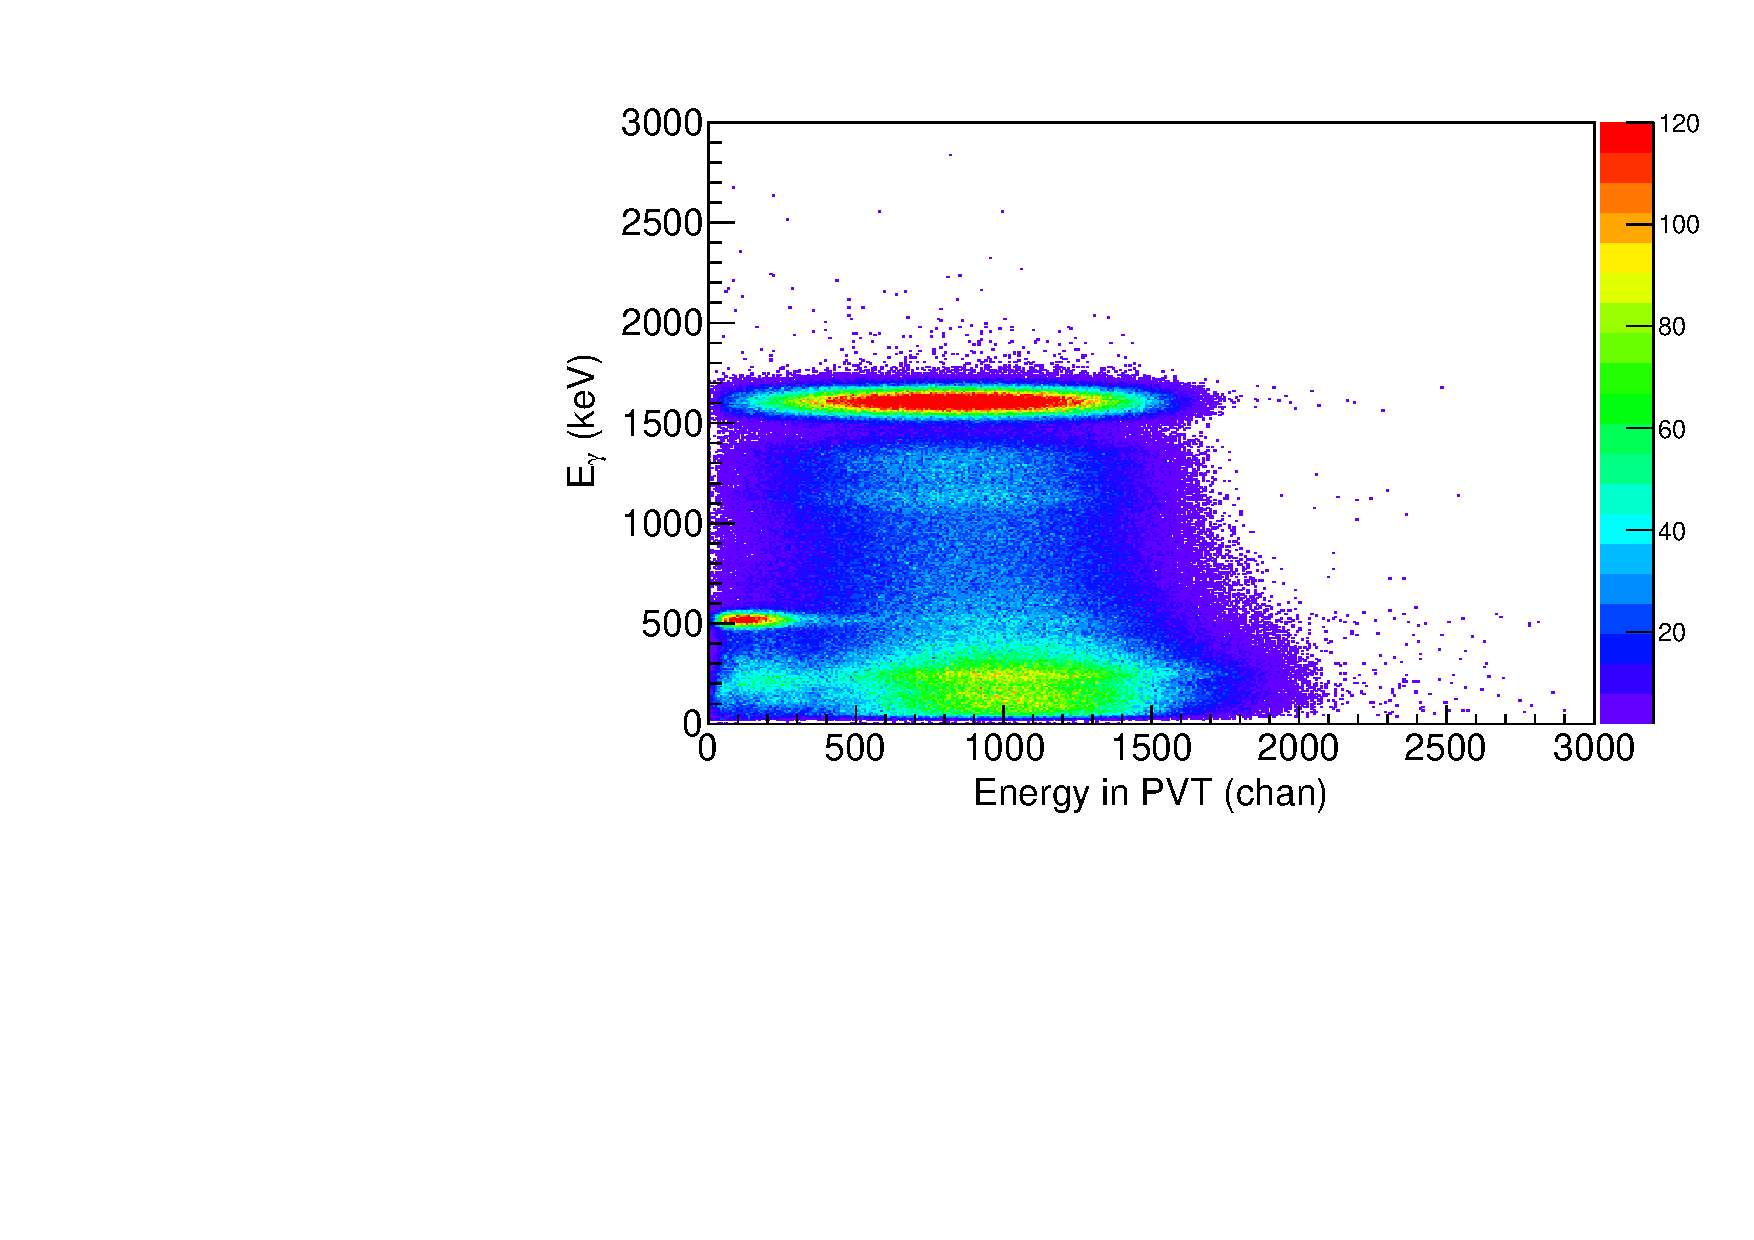
\includegraphics[width=0.78\textwidth]{fig_2Dh.pdf}}
	\caption{The 511 blob can be seen in this graph}
	\label{fig:2DGraph}
\end{figure}

\begin{figure}[!htb]
	\centerline{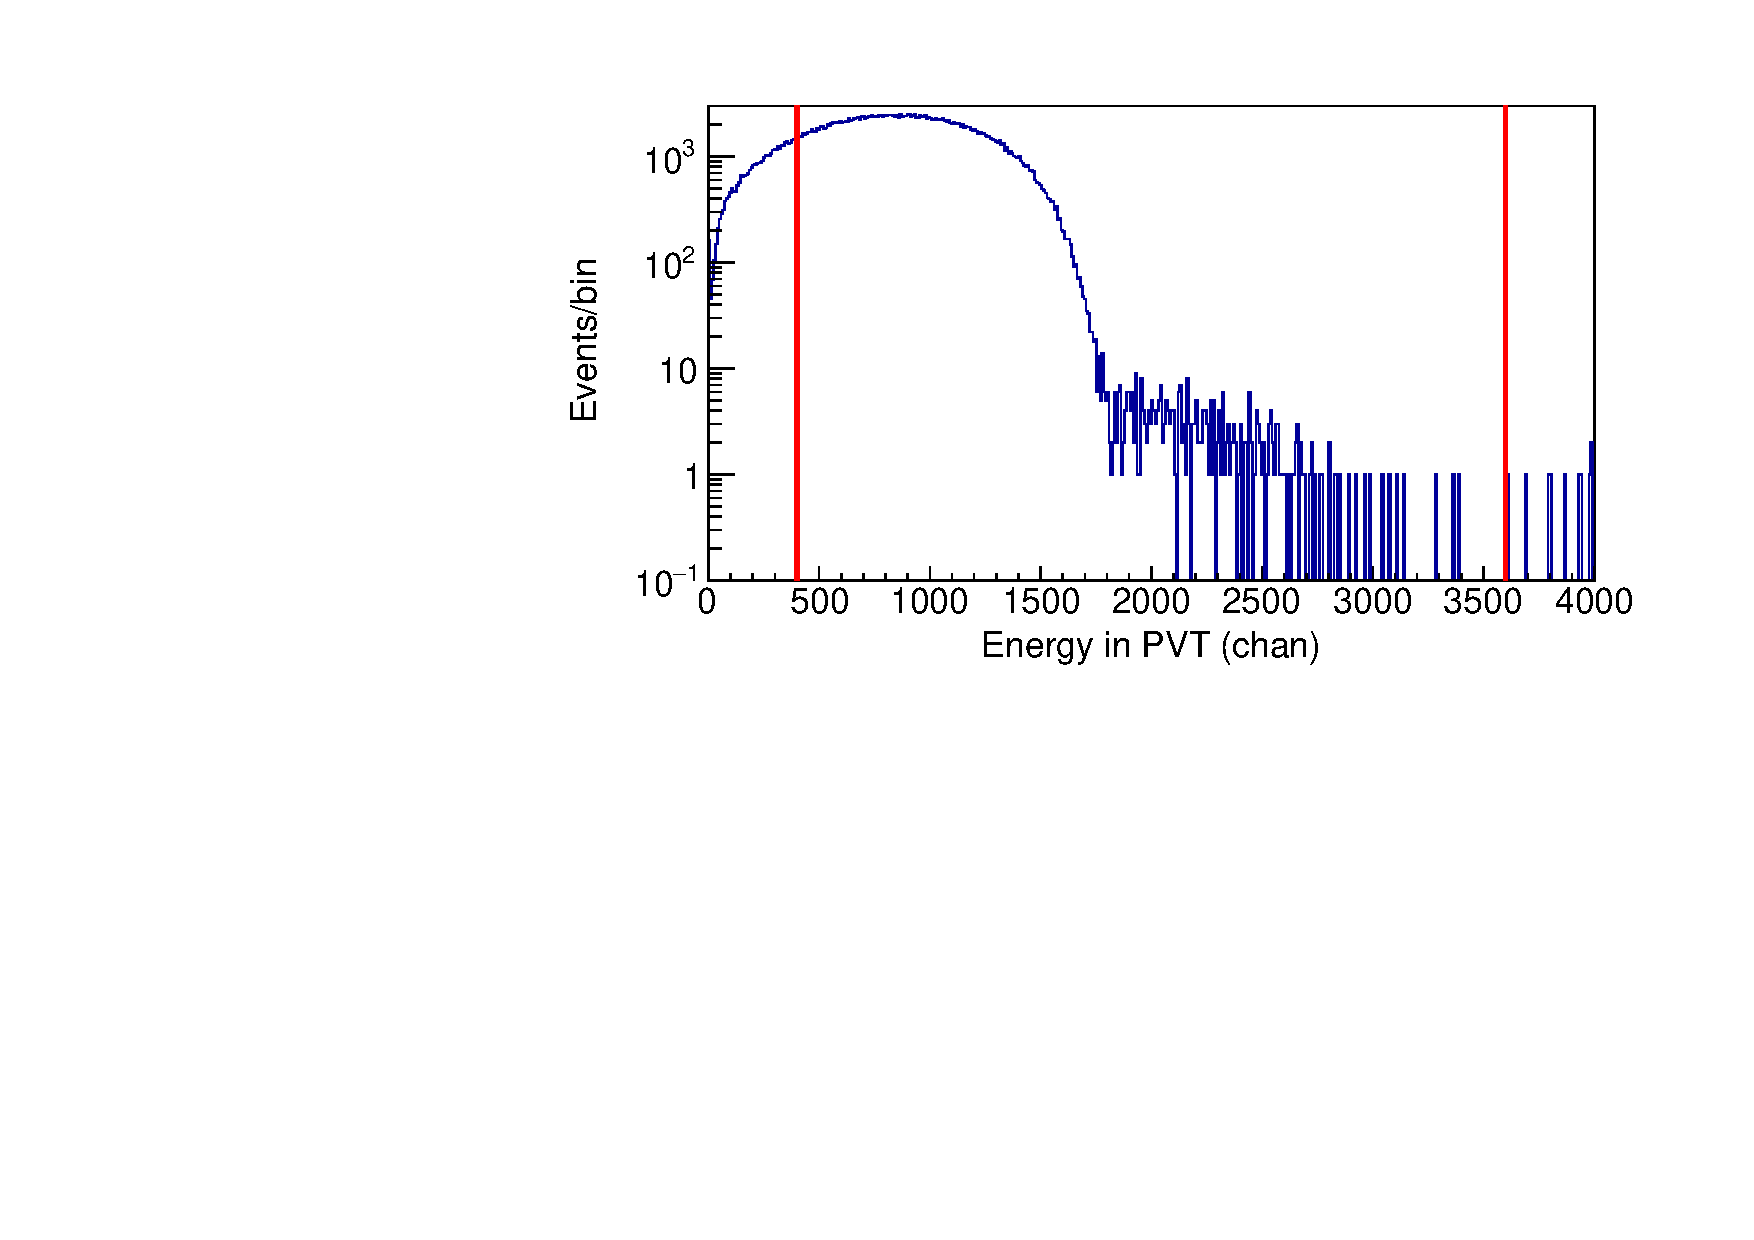
\includegraphics[width=0.78\textwidth]{fig_betaSpec.pdf}}
	\caption{The lower beta cut is selected to be above the 511 blob.}
	\label{fig:BetaGraph}
\end{figure}

\begin{figure}[!htb]
	\centerline{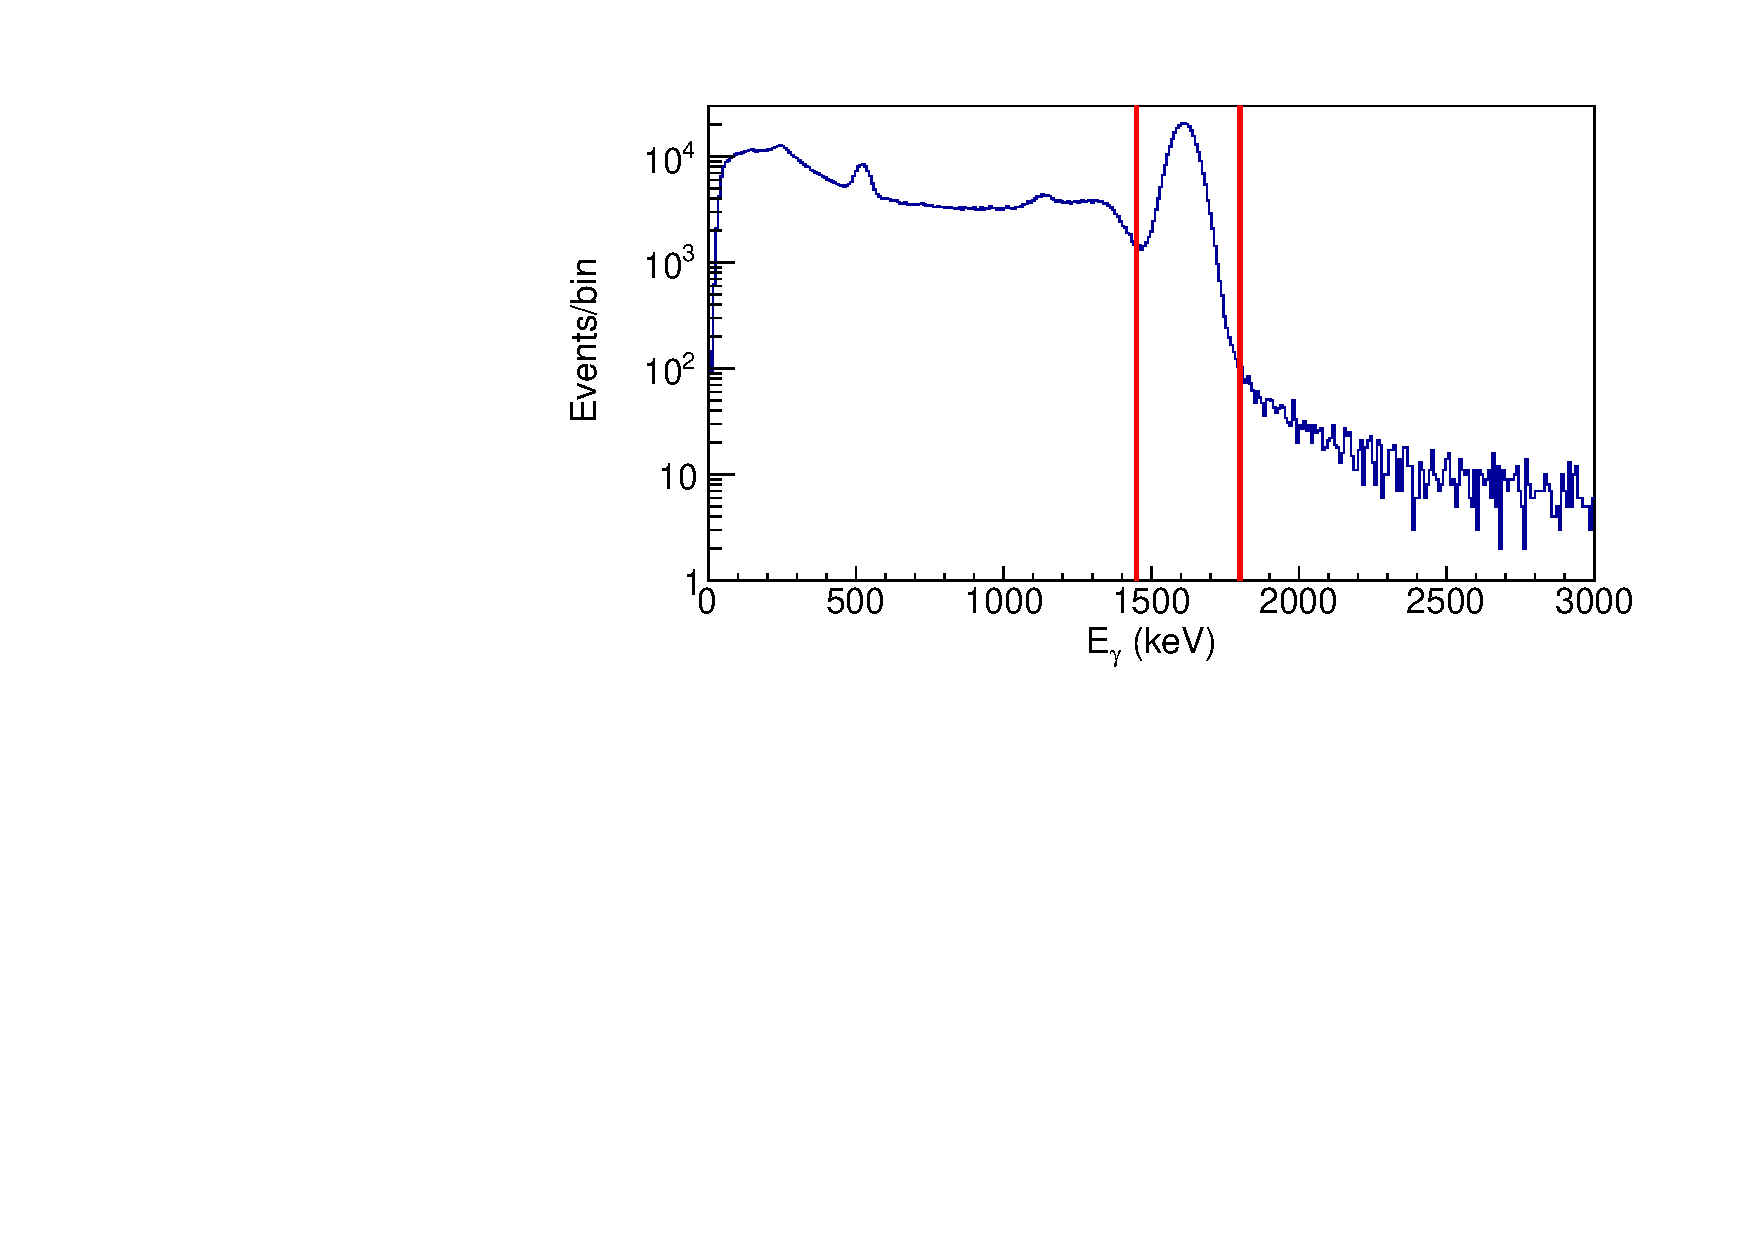
\includegraphics[width=0.78\textwidth]{fig_gammaSpec.pdf}}
	\caption{The wide cuts are to reduce the effect of the rate dependent gain.}
	\label{fig:Gammaraph}
\end{figure}

Hard coded gates were used for to select in the beta window for the PVT run sets.
Each different data set had a different energy window due to the gain shifts.
A sample spectrum with the gates can be seen in Figure \ref{fig:BetaGraph}.
This spectrum is put in coincidence with the gamma spectra. 
The lower beta cut was selected to cut out the 511 beta spectram as seen in Figure \ref{fig:2DGraph}.
When gated around that energies, the resulting gammas measured by the large CsI(Na) detectors are consistent with $^{10}$C and $^{11}$C.
This comes from the break-up of the plastic. 

The set of runs before the limiter box was installed have a gain shift within each run.
This causes the half-life to vary greatly with the beta cut.
As the beta gates are moved, different counts move across it over the time interval, causing a change in lifetime. 
Only the runs after the installation of the limiter box were used for the half-life analysis. 
This excluded the first and second sets of data.

%For the CsI(Na) implantation detector set, an additional complication occurs.
%Due to the afterglow of crystal, the gain of the detector depends on the rate.
%This causes all runs to have a greatly varying half-life as a function of the beta gates.
%Due to this, the CsI(Na) runs were not used in this analysls.
%
A time difference condition was set by building a spectrum of the time differences between the implant detector's event and one of the four gamma detector's events. 
The peak of this time difference spectrum was found, and an interval of $\pm$150 ns  was use for this gate.
A sample time difference spectrum can be seen in Figure \ref{fig:timediff}

\begin{figure}
	\centerline{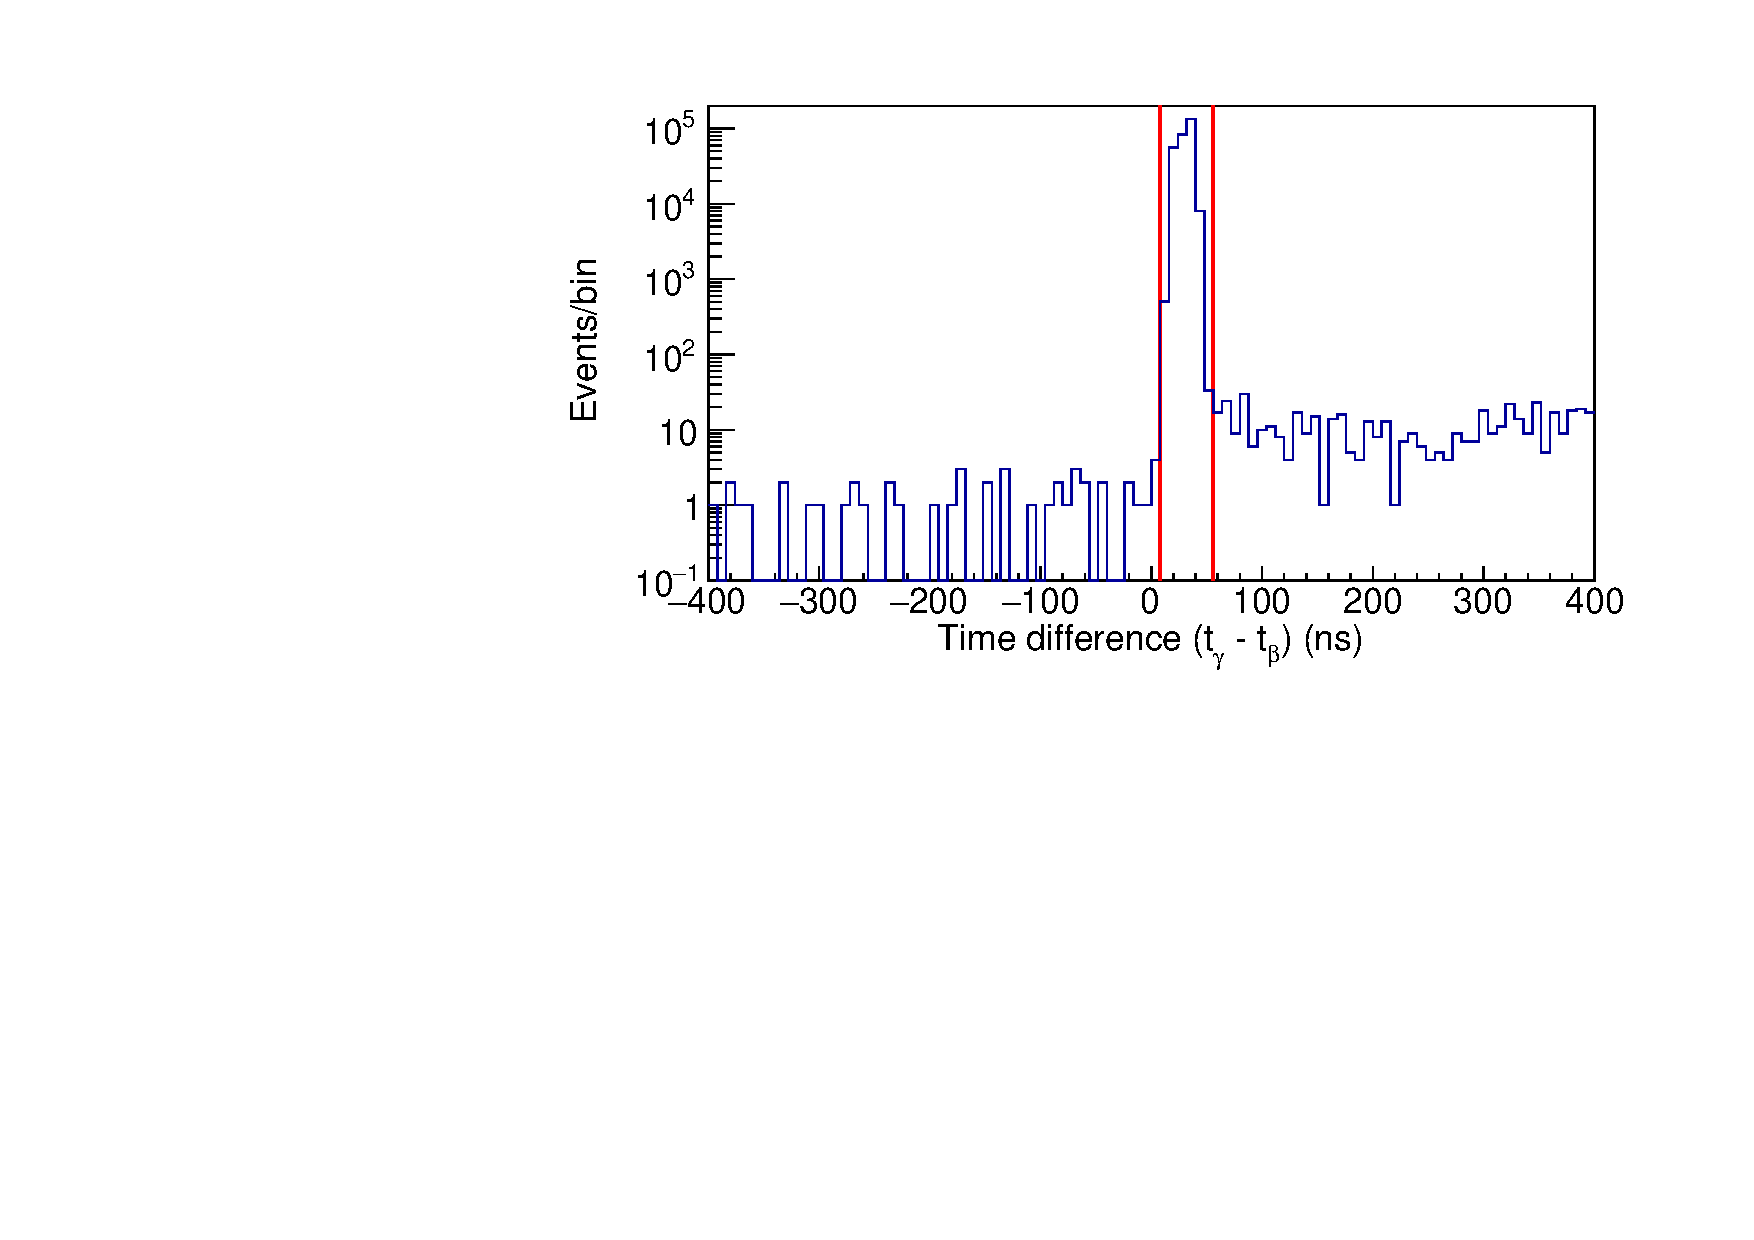
\includegraphics[width = 0.88\textwidth]{fig_tbgSpec1.pdf}}	
	\caption{This is a gamma and beta energy filted spectrum of the time difference between the up detector and the PVT implant detector.
		The tail on the right side of the large peak is due to pile up.
		The nominal time cuts are shown in red, while the narrow time cuts are shown in green.
		The green time cuts were used in systematic effect studies.} 
	\label{fig:timediff}
\end{figure}


The time signals for the outer four gamma detectors were used for the half-life analysis.
This gave 4 independent measurements of the half-life per run. 
Only full decay cycles were used. 
This was done by finding the last beam on and putting a condition on the run time of the events.
The decays where the up detector stopped counting were ignored, as there were few enough that they did not make a difference. 

The dead time was corrected using measured rates and a dead time of 464 ns for the implant detector and 656 ns for the gamma detectors.  
The dead time was measured by building a spectrum of the time difference between consecutive time stamps.
The lowest time difference was taken as the dead  time. 
This was checked using the light pulser in the PVT detector.
For each gamma detector, a spectrum of the energy-filtered rate was built.
The unfiltered implantation detector rate and gamma rate was built.
Using the uncorrected rates as an input, the gamma detector rate was corrected for bin by bin.
After the correction to the gamma detector rate, the rates were stacked up again to make one decay curve.
Once the decay spectra were put in coincidence and stacked up, it was fit with equation \ref{eq:fit-function}

%
\begin{equation}
	f(t) = a\exp{(-t/\tau)}
	\label{eq:fit-function}
\end{equation}
%
where $a$ and $\tau$ are the free parameters and $T_{1/2} = \frac{\ln{2}}{\tau})$. 
The decay curves were fit from 1.5 seconds past the beam on time to 1.5 second from the end of the decay time. 
The fitting method used was the log likelyhood method. 
The 60 second decay run up detector result is shown in Figure \ref{fig:60secdecay}.
From this run, it is seen that the spectra does not decay back down to the background. 
The lack of background parameter in equation \ref{eq:fit-function} comes from this observation. 

\begin{figure}[!htb]
\centerline{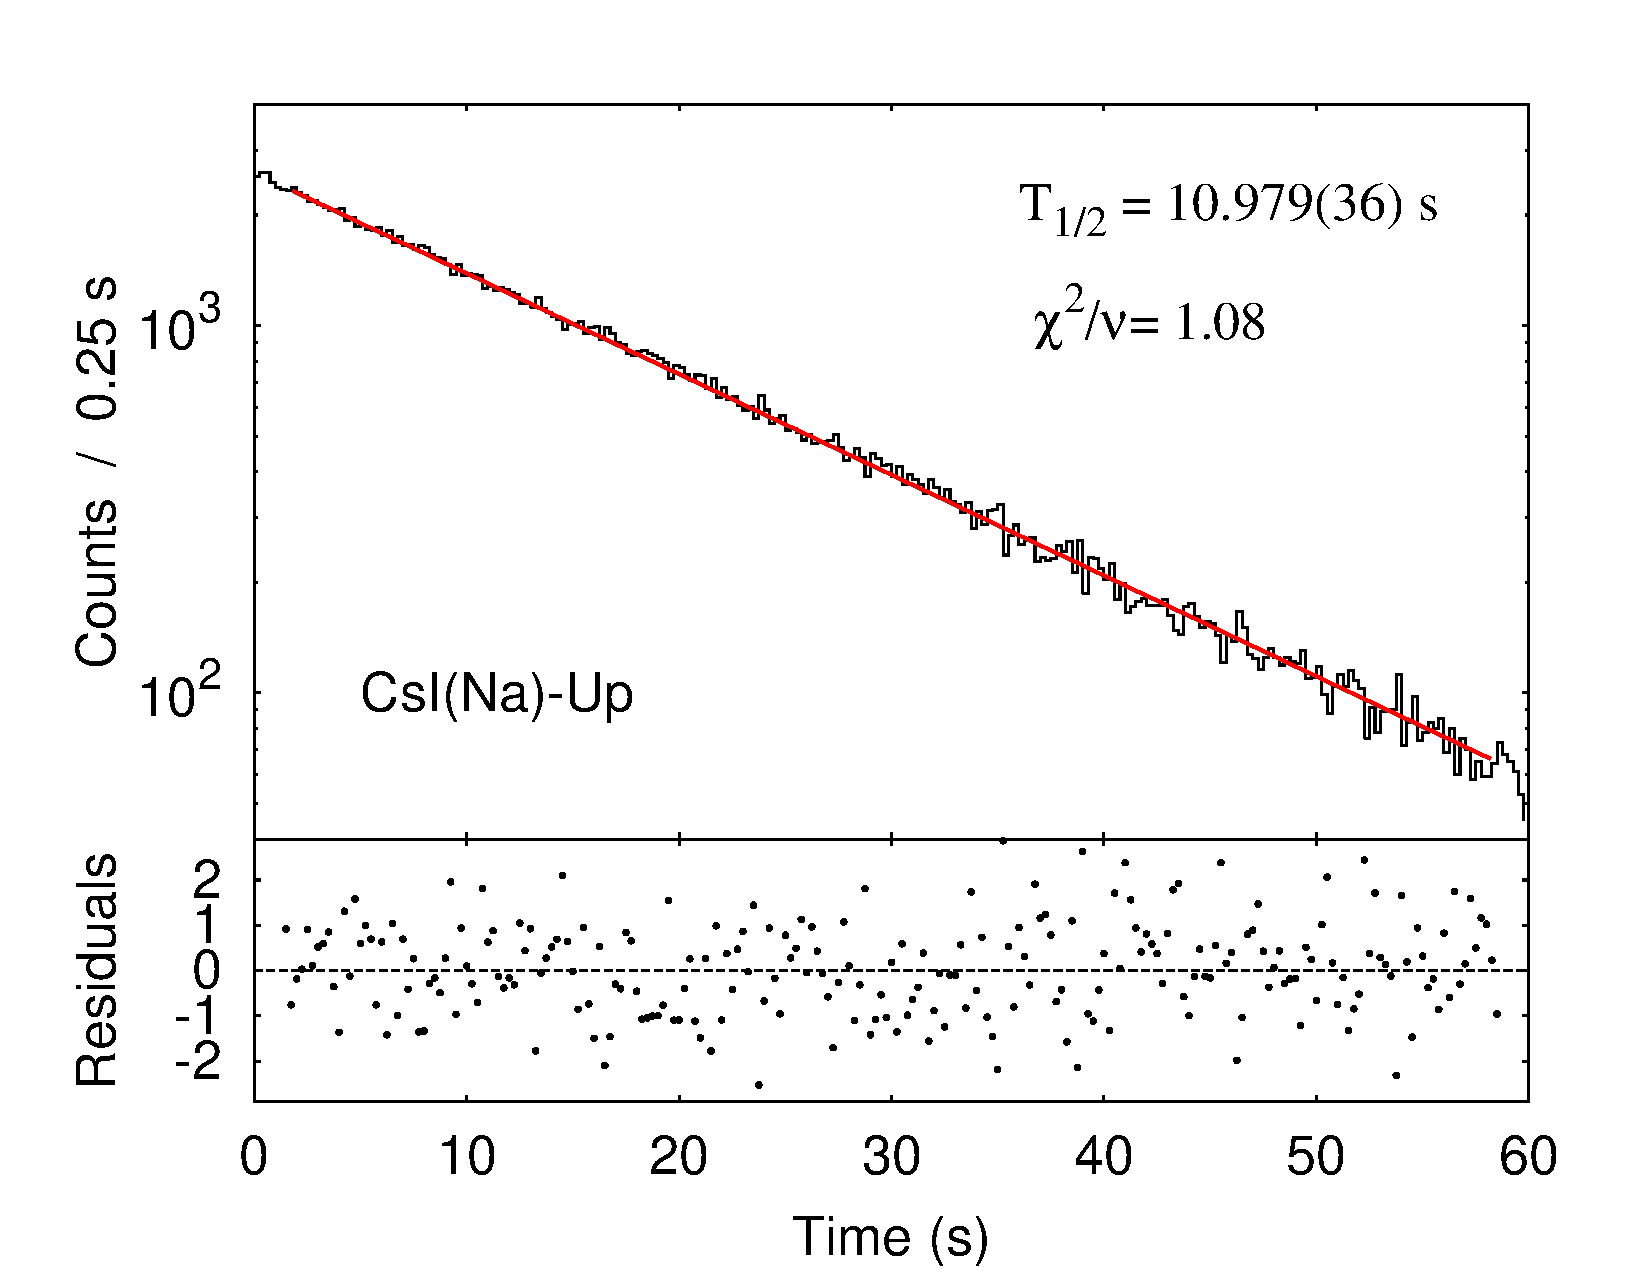
\includegraphics[width=0.88\textwidth]{fig_decaySpec.pdf}}
\caption{The decay spectrum from the up gamma detector is shown on the top graph.
	The red line is the exponential fit. 
	The bottom graph shows the residuals from the fit. 
	}
\label{fig:60secdecay}
\end{figure}


The decay spectra were built run by run, and the resulting fitting results were averaged together. 
Runs with a p-value less than 0.05 were considered statistically insignificant and thrown out.
After all the significant half-lives were collected, the average of them all was taken.
Several systematics were then looked at.

The first systematic effect is the effect of background.
To estimate the effect of background, each run's four spectra from the gamma detectors  was fit simultaneously. 
The equation used was equation \ref{eq:fit-function} with a linear background parameter added.
For this fit, the four spectra were assumed to have an equal half-life.
The background rate and initial rate, however, were assumed to be independent for each spectrum.
The difference of the half-lives between the two fitting methods was then divided by the square root of the sum of the squares of errors.
This normalized difference was compared to Monte Carlo results.

A Monte Carlo was written with a similar procedure done on spectra with a set, known background. 
Four spectra with a fixed and known background rate were generated.
They were fit with the two different methods, and the half-lives of each recorded.
Twenty or forty of these runs were generated, and the average of half-lives recorded.
The number of total statistics in each set of spectra was set to be equal to the number of filtered events in the data.
The difference of the two half-lives was divided by the total error of both methods.
This procedure was repeated 500 times to get a spectrum of these differences to compare to experiment. 

The time difference spectrum and the energy spectra can be used to argue for no background. 
Looking at Figure \ref{fig:timediff}, it can be seen that on the left side of the large peak, there are very few counts.
It can also be seen that the prompt peak in the center contains most of the counts, while there is a long tail on the right side of the peak.
This tail is due to pile up. 
An event in the beta window piles up with another event later in time. 
The second event is read by a gamma detector, but is correlated with the first event, causing the large time difference.
The time spectrum changes if the beta spectrum is cut in different ways.

In the gamma beta spectrum, it can be seen that there is no background events aside from the 511 blob.
This is due to the presence of $^{10}$C and $^{11}$C.
When the detectors are put into tripple and quadruple coincidence, the gamma rays of those isotopes appear.
There are no gamma rays in the 1620 keV window which was filtered on..
The only coincidence possible is if there is pile up into that window along with a beta event.
The estimate of those events is shown on the left side of the peak in the time difference figure shown in Fig. \ref{fig:timediff}  

The dead time is overcorrected above.
Due to pile up, some of the pile up events are not totally lost.
Some of the events thought to be missing just got shuffled around.
This is a problem due to the fact that energy gates are imposed.
To estimate the size of this effect, two different time cuts were compared.
A 48 ns time cut around the peak, shown in green in Figure \ref{fig:timediff}, was compared to the normal 300 ns time window.
Half the difference of these two effects was added as a systematic effect.	 

For each pair of detectors, there were four conditions: two for each the implant and gamma detectors. 
For the gamma cuts, the edges of the gates were varied $\pm$ 5 keV in each direction for each cut.
The upper beta cut was varied plus or minus 100 channels.
The lower beta cut was scanned with 6 different values going evenly from the initial lower beta cut to the peak of the spectrum.
Moving the lower beta cut also effects the dead time correction.
In order to disentangle the two, the lower beta cut was varied with two different time difference conditions.
The location where the difference between the two calculations blows up is where the effect of the lower beta cut starts being swamped by the effect of the pile up.
This is limit of where the lower beta cut was scanned.
All four of these conditions were varied independently, and the procedure of generation the spectrum and fitting the decay curves was done.
Half the resulting range of half-life values was taken to be a systematic uncertainty.
	
The fitting range of the decay spectra was varied. 
The start of the fit was varied bin by bin up to 6.5 seconds into the decay spectrum.
The end of the fit was varied the other way to cut out the end of the decay spectrum.
Since there was no noticable systematic effect, there was no increase in error associated with this effect.

%%%%%%%%%%%%%%%%%%%%%%%%%%%%%%%%%%%%%%%%%%%%%%%%%%%%%%%%%%%%%%%%%%%%%%%%%%%%
\section{Result and discussion}
\label{sec:result}

The PVT runs are shown in Figure \ref{fig:PVT2by2}

\begin{figure}[!htb]
	\centerline{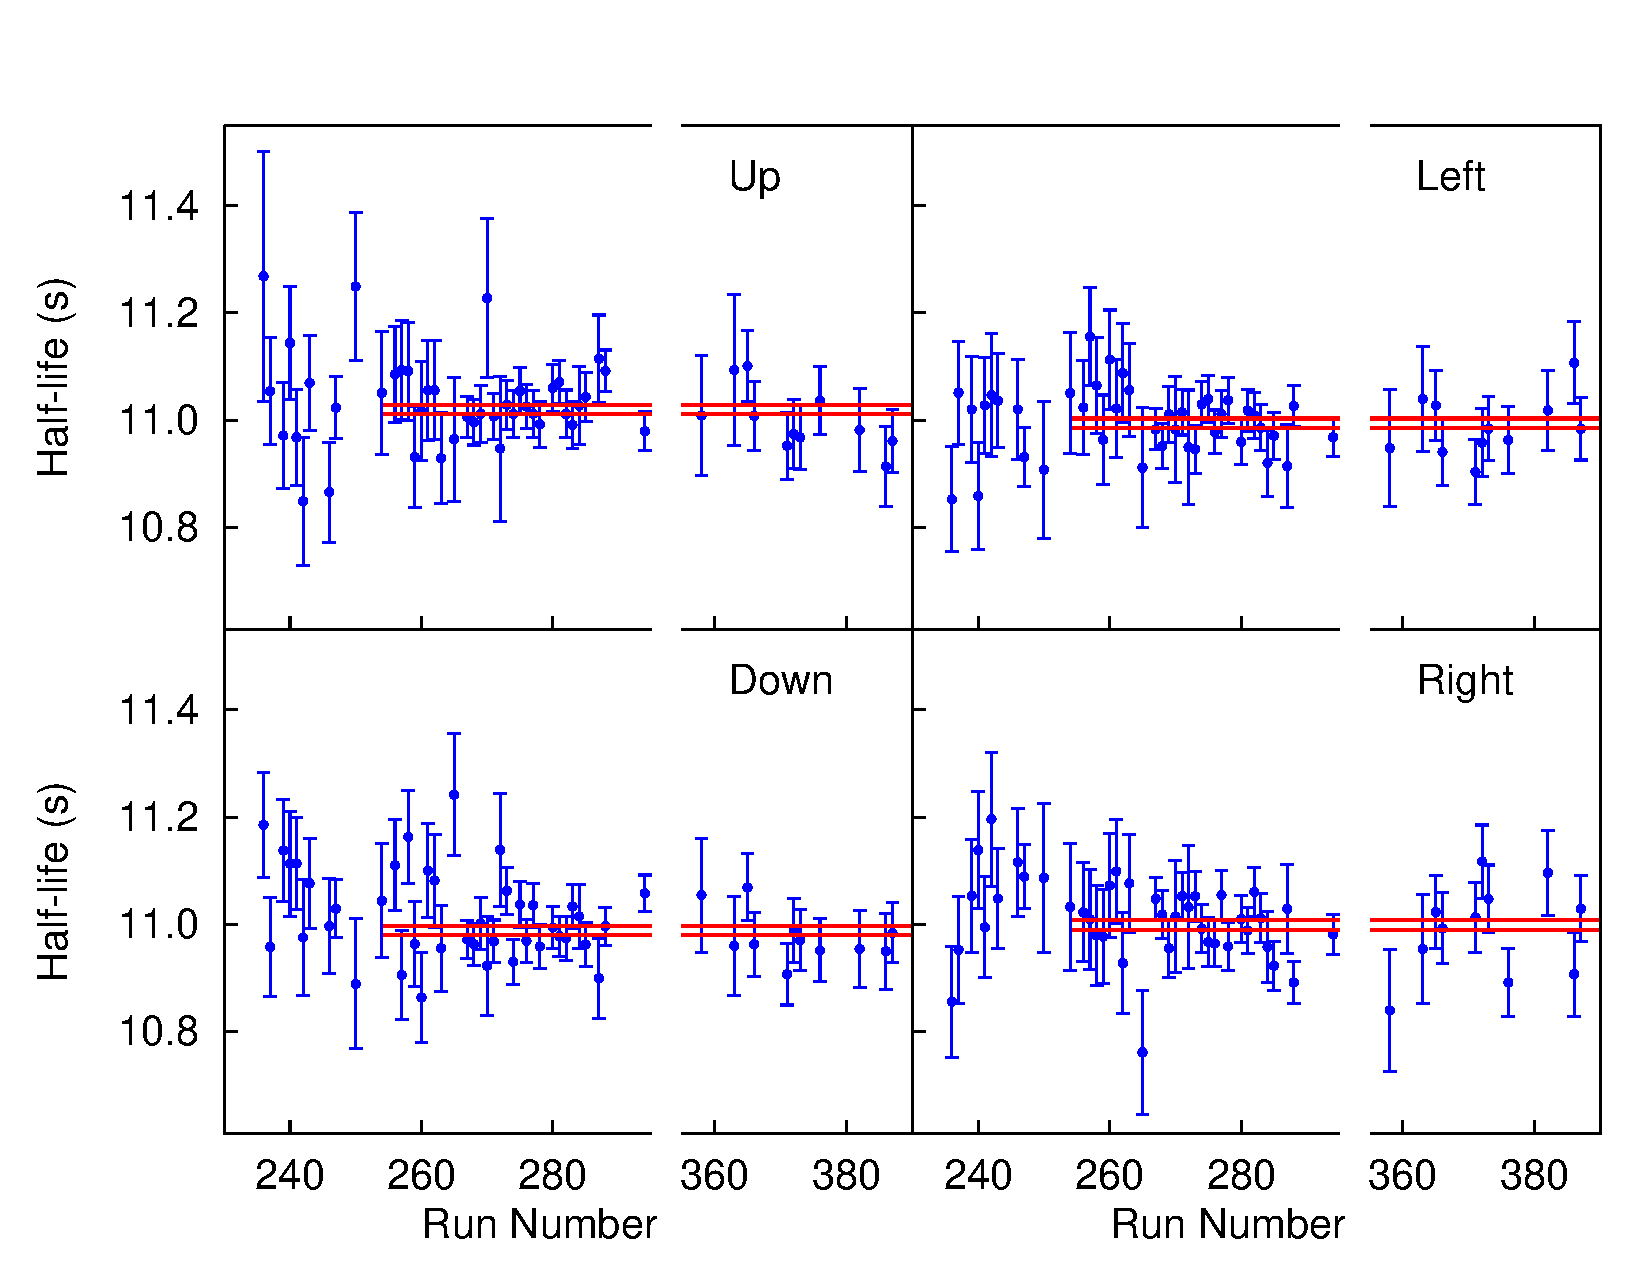
\includegraphics[width=0.88\textwidth]{fig_halfLives.pdf}}
	\caption{The red lines show the results of the fits over the runs that were used.
		 The additional half-lives shown are excluded to reasons discussed previously. 
		}
	\label{fig:PVT2by2}
\end{figure}

The results for the PVT runs are shown in  in table \ref{tab:PVTTable} for the PVT runs.
%\begin{center}
	\begin{table}[!hbt]
			\caption{The PVT runs}
			\begin{tabular}{l|r|r}
			Detector & Half-Life & Error \\ \hline
			Up & 11.0215 & 0.0090 \\
			Left & 10.9988 & 0.0090 \\
			Down & 10.9925 & 0.0085 \\
			Right & 11.014 & 0.0095 
			\end{tabular}
			\label{tab:PVTTable}
	\end{table}
%\end{center}

The size of the systematic errors investigated are shown in table \ref{tab:SysTable} 

%\begin{center}
\begin{table}[!hbt]
\caption{Systematic Errors}
	\label{tab:err-budget}
		\begin{tabular}{l|r|r}
		Source & Correction [ms] & Uncertainty [ms] \\ \hline
		Dead-time & 0.0 & 0.24 \\
		Lower beta cut variation & 0.0 & 2.32 \\
		Upper beta Cut variation & 0.0 & 0.83 \\
		Lower gamma cut variation & 0.0 &  0.15\\
		Upper gamma cut variation & 0.0 & 0.05 \\ 
		Realitive time cut & 2.25 & 2.25 \\
		Binning & -0.30 & 0.30
		\end{tabular}
	\label{tab:SysTable}
\end{table}
%\end{center}
After the dead time correction, the value of the half-life from the CsI(Na) implant detector runs was found to be 11.052 $\pm$ 0.044 (stat) $\pm$ 0.034 (syst) s.

%%%%%%%%%%%%%%%%%%%%%%%%%%%%%%%%%%%%%%%%%%%%%%%%%%%%%%%%%%%%%%%%%%%%%%%%%%%%
\section{Conclusion}
\label{sec:conclusion}

The half-life measured is most consistent with some previous measurements of a half-life of about 11 s. 
This can be seen in Figure \ref{fig:ideogramfinal}.
This measure disagrees with the most recent measurements.

\begin{figure}[!htb]
\centerline{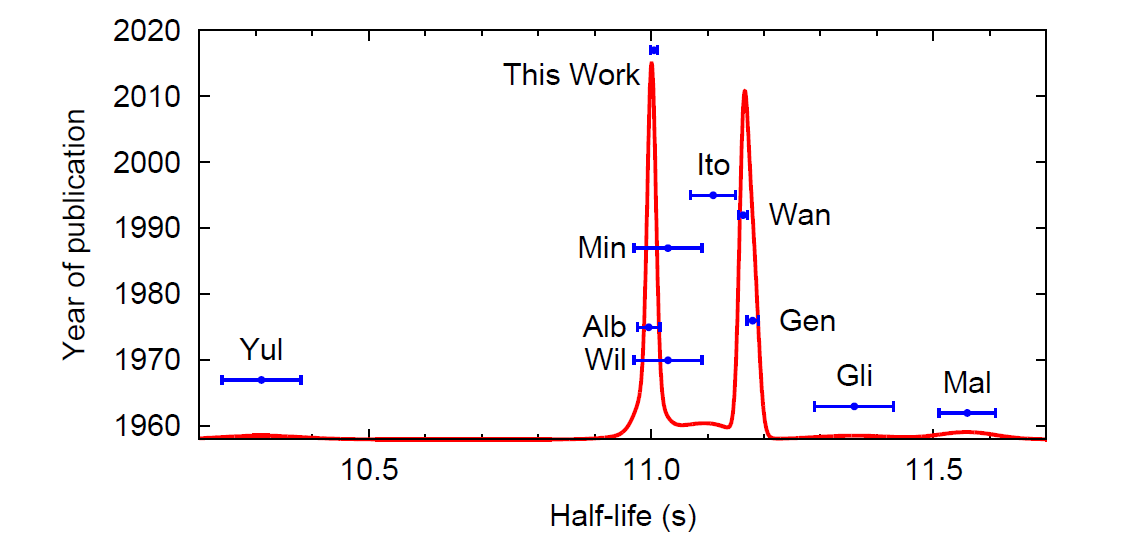
\includegraphics[width=0.88\textwidth]{fig_ideogramAfter.png}}
\caption{A scatter plot of (a) previous values with this work added.
	 The labels correspond to: Mal~\cite{Mal62}, Gli~\cite{Gli63},
	Yul~\cite{Yul67}, Wil~\cite{Wil70}, Alb~\cite{Alb75}, Gen~\cite{Gen76},
	Min \cite{Min87}, Wan~\cite{Wan92} and Ito~\cite{Ito95}.}
\label{fig:ideogramfinal}
\end{figure}

Several things about the data set were discovered.
It was learned that there were contaminates coming from the fragmentation of the $^{12}$C in the plastic scinttilator.
The beta decaying products could be a cause of why the beta spectrum for the PVT detector looks so odd.
It was also discovered that the rate dependent gain effect in the CsI(Na) implant detector is significant.
Before doing this measurement, it was assumed that the low rates would make that effect negligable.
It was learned that after the coincidence, the amount of background left in the spectrum is negligable, and that we have no contaminates in the beam.


%%%%%%%%%%%%%%%%%%%%%%%%%%%%%%%%%%%%%%%%%%%%%%%%%%%%%%%%%%%%%%%%%%%%%%%%%%%%
%Bibliography

%%%%%%%%%%%%%%%%%%%%%%%%%%%%%%%%%%%%%%%%%%%%%%%%%%%%%%%%%%%%%%%%%%%%%%%%%%%%
%%%%%%%%%%%%%%%%%%%%%%%%%%%%%%%%%%%%%%%%%%%%%%%%%%%%%%%%%%%%%%%%%%%%%%%%%%%%
